\subsection{Ve spojení s bezpečností v počítačových sítích definujeme tyto pojmy}
\begin{itemize}
\item \textbf{Utajení} (confidentality) – posluchač na kanále datům nerozumí.
\item \textbf{Autentizace} (authentication) – jistota, že odesílatel je tím, za koho se vydává.
\item \textbf{Integrita} (integrity) – jistota, že data nebyla na cestě zmodifikována.
\item \textbf{Nepopiratelnost} (non-repudiation) – zdroj dat nemůže popřít jejich odeslání.
\end{itemize}

\subsection{Útoky}
Cílem všech typů útoků je nějakým způsobem ublížit uživateli, často ve formě: zahlcení sítě packety, narušení konfigurace nastavení, zabránění uživateli v přístupu ke službě, \textbf{zatížení CPU}, pád OS. Typy útoků:
\begin{itemize}
	\item \textbf{ARP dotazy} -- falšování ARP odpovědí (falešný překlad IP-to-MAC). \textbf{Oprava} užitím statických ARP záznamů.
	\item \textbf{Routing protocol} -- falšování routovacích informací propagovaných routovacím protokolem (RIP atd). Oprava 	\textbf{filtrováním} zdrojů routovacích informací.
	\item \textbf{Switchované sítě} -- proti přetížení přepínací tabulky. Oprava užitím limitování počtu MAC na portu, statickým 	listem povolených MAC.
	\item \textbf{Brute Force} -- zadávání hesel pomocí hrubé síly.
	\item \textbf{Denialenial of service (DoS)} - cílem útočníka vyčerpání systémových prostředků (paměť, CPU, šířka pásma) síťového prvku nebo serveru a jeho zhroucení nebo změna požadovaného chování.
\begin{itemize}
	\item \textbf{Smurf} -- zahlcení cíle ICMP pakety (ping), jejich zpracování mívá někdy přednost před běžným provozem; útočník pošle žádost o ping všem (broadcast) a jako odesilatele uvede cíl útoku. \textbf{Řešení:} packetové filtry.
	\item \textbf{SYN flood} -- neustálé navazování TCP spojení (příznak SYN), server alokuje prostředky a pošle (SYN-ACK) a čeká na odpověď, které se nedočká. \textbf{Řešení:} zkrácení doby čekání na odpověď.
\end{itemize}
	\item \textbf{Distributed DoS (DDoS)} -- DoS útok je vedený z mnoha stanic, které byli již před tím napadeny a nyní jsou využity k tomuto útoku. Je obtížně blokovatelný kvůli přístupu mnoha stanic.
\end{itemize}

\subsection{Filtrování provozu}
\subsubsection{Paketové filtry (nestavové)}
\textbf{Filtrování probíhá dle informací v hlavičce 3 a 4 vrstvy}. Pravidla udávají, ze které adresy a portu na kterou adresu a port může být paket procházející rozhraním routeru propuštěn. Na routerech CISCO je realizován jako \textbf{Access Control List (ACL)} prostřednictvím sekvence záznamu, které povolují/zakazují přenos paketu, které odpovídají daným kritériím. Samotný paketový filtr je rychlý, nenáročný na systémové zdroje, ale úroveň kontroly je relativně malá.

\subsubsection{Stavový firewall}
(též stavový paketový filtr, anglicky stateful firewall) odděluje důvěryhodnou (interní) síť od nedůvěryhodné (externí) sítě. Funguje stejně jako jednoduchý paketový filtr, ukládá \textbf{navíc ale i informace o povolených spojeních}, podle kterých pak může rozhodovat, zda procházející pakety patří do již povoleného spojení a mohou být propuštěny nebo zda musí znovu projít kontrolou. Firewall je \textbf{velmi rychlý}, poskytuje slušnou úroveň zabezpečení a snazší konfiguraci.  Poskytuje urychlené zpracování paketu již povoleného spojení. Obdobou stavového firewallu je \textbf{nestavový firewall}, který se rozhoduje pouze na základě informací obsažených v konkrétním paketu (pracuje na nižší síťové vrstvě ISO/OSI modelu) a aplikační firewall, který pracuje naopak na vyšší síťové vrstvě. 
\\\\
\noindent\makebox[\textwidth]{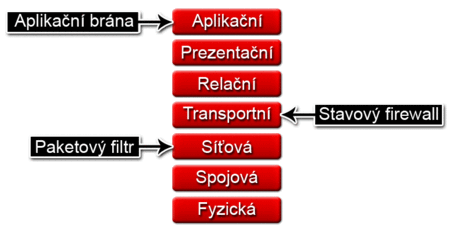
\includegraphics[width=8cm]{assets/7_filter}}

\subsection{Virtuální privátní síť }
(zkratka VPN, anglicky virtual private network) je v informatice prostředek k \textbf{propojení několika počítačů prostřednictvím (veřejné) nedůvěryhodné počítačové sítě}. Lze tak snadno dosáhnout stavu, kdy spojené počítače budou mezi sebou moci komunikovat, jako kdyby byly propojeny v rámci jediné uzavřené privátní (a tedy důvěryhodné) sítě. Při navazování spojení je totožnost obou stran ověřována pomocí \textbf{digitálních certifikátů}, dojde k autentizaci, vytvoření duplexního kanálu, veškerá komunikace je šifrována, a proto můžeme takové propojení považovat za bezpečné.

\subsection{Šifrování}
\subsubsection{Symetrické šifrování}
Pro šifrování i dešifrování se používá \textbf{pouze jeden klíč}, který musí mít všichni účastníci, kteří chtějí data šifrovat nebo dešifrovat. \textbf{Nebezpečí hrozí při distribuci }tohoto klíče, který pokud bude prozrazen tak všichni účastníci musí začít používat nový klíč.  Šifrování je \textbf{rychlé} a \textbf{jednoduché} pro implementaci (možná implementace přímo v HW). Nejznámější \textbf{AES},	 \textbf{DES}, \textbf{3DES}, \textbf{IDEA}. \textbf{DES} již dnes není bezpečný, používá se \textbf{3DES}, který \textbf{DES} zašifruje 3x po sobě.
\\\\
\noindent\makebox[\textwidth]{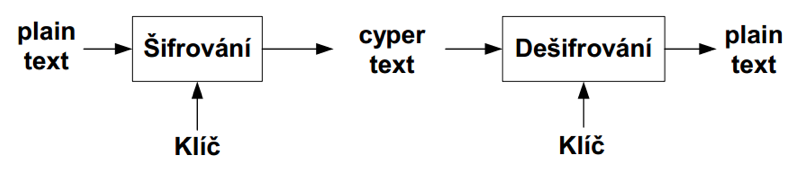
\includegraphics[width=10cm]{assets/7_symetric}}

\subsubsection{Asymetrické šifrování}
Podstatou je \textbf{generace dvou šifrovacích klíčů}, které spolu spolupracují. Tyto klíče se vzájemně matematicky doplňují a je možné oba použít jak pro dešifrování tak šifrování. Veřejný klíč je volně šiřitelný pro všechny, kteří chtějí šifrovat posílaná data. Soukromý klíč je tajný a je pouze pro potřebu pro dešifrování toho, co bylo zašifrováno veřejným klíčem. Uživatel tedy pro šifrovanou komunikaci potřebuje oba klíče. Výhodou je, že\textbf{ není třeba veřejný klíč speciálně ukrývat} (je vyřešena metoda distribuce), pouze je třeba zajistit mechanizmus proti modifikaci veřejných klíčů při přenosu - \textbf{certifikovaná autorita (CA)} klíč digitálně podepisuje. Nevýhodou je, že v porovnání se symetrickým je \textbf{pomalejší} z důvodu použitých matematických funkcí. Asymetrické systémy jsou např. \textbf{RSA} nebo \textbf{DSA}. Stupeň \textbf{bezpečnosti se odvíjí od délky} použitého klíče.
\\\\
\noindent\makebox[\textwidth]{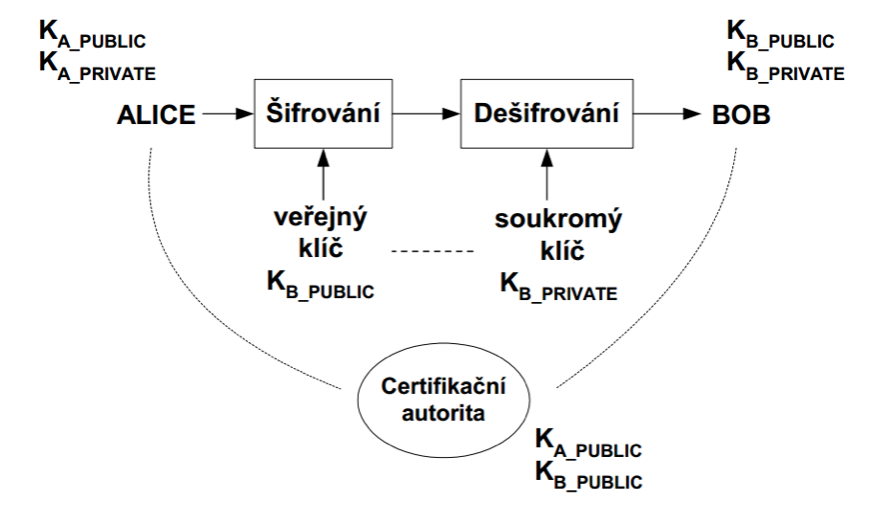
\includegraphics[width=10cm]{assets/7_asymetric}}


\subsubsection{Certifikační autorita}
\begin{itemize}
	\item Entita, které je důvěřováno.
	\item Registruje (podepsané) veřejné klíče.
	\item První kontakt s certifikační autoritou \textbf{musí proběhnout osobně }(získání dvojice podepsaný veřejný-privátní klíč).
	\item Veřejný klíč certifikační autority musí být \textbf{důvěryhodným} způsobem zaveden do každého systému.
\end{itemize}


\subsubsection{Autentizace}
Je proces ověření proklamované identity subjektu. Probíhá nejčastěji jednou ze tří metod:
\begin{itemize}
\item Řekneme něco, co známe (\textbf{heslo}, PIN)
\item Ukážeme něco, co máme (ID karta, \textbf{hardwarový klíč})
\item Necháme systémem změřit něco našeho (\textbf{biometrické údaje}, otisk prstů, sítnice)
\end{itemize}
Existuje \textbf{několika stupňové ověření}, například kombinací PIN a biometrických údajů. Po ověření identity následuje autorizace což je souhlas k provedení operace či umožnění přístupu. \textbf{Často se používá v souladu s šifrováním:}
\begin{itemize}
\item U \textbf{symetrického} odesílatel šifruje uživatelské jméno sdíleným klíčem a příjemce kontroluje platnost tohoto uživatelského jména.
\item U \textbf{asymetrického} se užívá digitálních podpisů Certifikační autority.
\end{itemize}



\subsection{Zabezpečení na jednotlivých vrstvách OSI-RM }
\begin{itemize}
	\item \textbf{L7} – S/MIME,
	\item \textbf{L4} – SSL (jen TCP),
	\item \textbf{L3} – IPSec (bezpečnostní rozšíření IP protokolu založené na autentizaci a šifrování každého IP datagramu) \textbf{nezávislé na aplikaci},
	\item \textbf{L2} – hop-by-hop, neefektivní.
\end{itemize}


\subsubsection{SSL}
Secure Sockets Layer, SSL (doslova vrstva bezpečných socketů) je protokol, resp. \textbf{vrstva vložená mezi vrstvu transportní} (např. TCP/IP) a \textbf{aplikační} (např. HTTP), která \textbf{poskytuje zabezpečení komunikace} šifrováním a autentizaci komunikujících stran.

Protokol SSL se nejčastěji využívá pro bezpečnou komunikaci s internetovými servery pomocí HTTPS, což je zabezpečená verze protokolu HTTP. Po vytvoření SSL spojení (session) je komunikace mezi serverem a klientem šifrovaná a tedy zabezpečená.

Ustavení SSL spojení funguje na principu \textbf{asymetrické šifry}, kdy každá z komunikujících stran má dvojici šifrovacích klíčů - veřejný a soukromý. Veřejný klíč je možné zveřejnit, a pokud tímto klíčem kdokoliv zašifruje nějakou zprávu, je zajištěno, že ji bude moci rozšifrovat jen majitel použitého veřejného klíče svým soukromým klíčem.

